% Graphic for TeX using PGF
% Title: /home/hayat/report_memoire/illustrations/key-value-nosql.dia
% Creator: Dia v0.97+git
% CreationDate: Sun Dec  2 15:37:59 2018
% For: hayat
% \usepackage{tikz}
% The following commands are not supported in PSTricks at present
% We define them conditionally, so when they are implemented,
% this pgf file will use them.
\ifx\du\undefined
  \newlength{\du}
\fi
\setlength{\du}{15\unitlength}
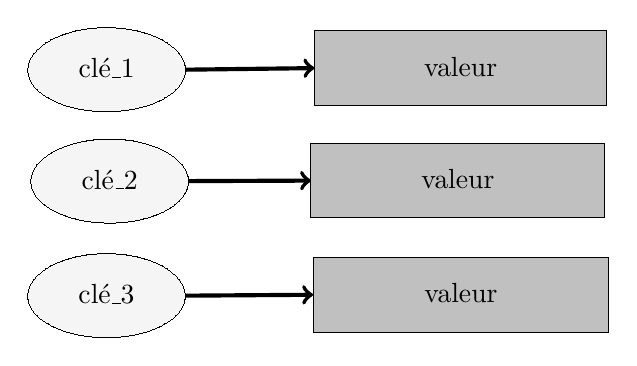
\begin{tikzpicture}[even odd rule]
\pgftransformxscale{1.000000}
\pgftransformyscale{-1.000000}
\definecolor{dialinecolor}{rgb}{0.000000, 0.000000, 0.000000}
\pgfsetstrokecolor{dialinecolor}
\pgfsetstrokeopacity{1.000000}
\definecolor{diafillcolor}{rgb}{1.000000, 1.000000, 1.000000}
\pgfsetfillcolor{diafillcolor}
\pgfsetfillopacity{1.000000}
\pgfsetlinewidth{0.000000\du}
\pgfsetdash{}{0pt}
\pgfsetmiterjoin
\definecolor{diafillcolor}{rgb}{0.960784, 0.960784, 0.960784}
\pgfsetfillcolor{diafillcolor}
\pgfsetfillopacity{1.000000}
\pgfpathellipse{\pgfpoint{7.950991\du}{7.987995\du}}{\pgfpoint{1.899011\du}{0\du}}{\pgfpoint{0\du}{1.012005\du}}
\pgfusepath{fill}
\definecolor{dialinecolor}{rgb}{0.000000, 0.000000, 0.000000}
\pgfsetstrokecolor{dialinecolor}
\pgfsetstrokeopacity{1.000000}
\pgfpathellipse{\pgfpoint{7.950991\du}{7.987995\du}}{\pgfpoint{1.899011\du}{0\du}}{\pgfpoint{0\du}{1.012005\du}}
\pgfusepath{stroke}
% setfont left to latex
\definecolor{dialinecolor}{rgb}{0.000000, 0.000000, 0.000000}
\pgfsetstrokecolor{dialinecolor}
\pgfsetstrokeopacity{1.000000}
\definecolor{diafillcolor}{rgb}{0.000000, 0.000000, 0.000000}
\pgfsetfillcolor{diafillcolor}
\pgfsetfillopacity{1.000000}
\node[anchor=base,inner sep=0pt, outer sep=0pt,color=dialinecolor] at (7.950991\du,8.182995\du){clé\_1};
\pgfsetlinewidth{0.000000\du}
\pgfsetdash{}{0pt}
\pgfsetmiterjoin
\definecolor{diafillcolor}{rgb}{0.960784, 0.960784, 0.960784}
\pgfsetfillcolor{diafillcolor}
\pgfsetfillopacity{1.000000}
\pgfpathellipse{\pgfpoint{8.024011\du}{10.672005\du}}{\pgfpoint{1.899011\du}{0\du}}{\pgfpoint{0\du}{1.012005\du}}
\pgfusepath{fill}
\definecolor{dialinecolor}{rgb}{0.000000, 0.000000, 0.000000}
\pgfsetstrokecolor{dialinecolor}
\pgfsetstrokeopacity{1.000000}
\pgfpathellipse{\pgfpoint{8.024011\du}{10.672005\du}}{\pgfpoint{1.899011\du}{0\du}}{\pgfpoint{0\du}{1.012005\du}}
\pgfusepath{stroke}
% setfont left to latex
\definecolor{dialinecolor}{rgb}{0.000000, 0.000000, 0.000000}
\pgfsetstrokecolor{dialinecolor}
\pgfsetstrokeopacity{1.000000}
\definecolor{diafillcolor}{rgb}{0.000000, 0.000000, 0.000000}
\pgfsetfillcolor{diafillcolor}
\pgfsetfillopacity{1.000000}
\node[anchor=base,inner sep=0pt, outer sep=0pt,color=dialinecolor] at (8.024011\du,10.867005\du){clé\_2};
\pgfsetlinewidth{0.000000\du}
\pgfsetdash{}{0pt}
\pgfsetmiterjoin
\definecolor{diafillcolor}{rgb}{0.960784, 0.960784, 0.960784}
\pgfsetfillcolor{diafillcolor}
\pgfsetfillopacity{1.000000}
\pgfpathellipse{\pgfpoint{7.949011\du}{13.432005\du}}{\pgfpoint{1.899011\du}{0\du}}{\pgfpoint{0\du}{1.012005\du}}
\pgfusepath{fill}
\definecolor{dialinecolor}{rgb}{0.000000, 0.000000, 0.000000}
\pgfsetstrokecolor{dialinecolor}
\pgfsetstrokeopacity{1.000000}
\pgfpathellipse{\pgfpoint{7.949011\du}{13.432005\du}}{\pgfpoint{1.899011\du}{0\du}}{\pgfpoint{0\du}{1.012005\du}}
\pgfusepath{stroke}
% setfont left to latex
\definecolor{dialinecolor}{rgb}{0.000000, 0.000000, 0.000000}
\pgfsetstrokecolor{dialinecolor}
\pgfsetstrokeopacity{1.000000}
\definecolor{diafillcolor}{rgb}{0.000000, 0.000000, 0.000000}
\pgfsetfillcolor{diafillcolor}
\pgfsetfillopacity{1.000000}
\node[anchor=base,inner sep=0pt, outer sep=0pt,color=dialinecolor] at (7.949011\du,13.627005\du){clé\_3};
\pgfsetlinewidth{0.000000\du}
\pgfsetdash{}{0pt}
\pgfsetmiterjoin
{\pgfsetcornersarced{\pgfpoint{0.000000\du}{0.000000\du}}\definecolor{diafillcolor}{rgb}{0.752941, 0.752941, 0.752941}
\pgfsetfillcolor{diafillcolor}
\pgfsetfillopacity{1.000000}
\fill (12.956200\du,7.050000\du)--(12.956200\du,8.850000\du)--(19.999950\du,8.850000\du)--(19.999950\du,7.050000\du)--cycle;
}{\pgfsetcornersarced{\pgfpoint{0.000000\du}{0.000000\du}}\definecolor{dialinecolor}{rgb}{0.000000, 0.000000, 0.000000}
\pgfsetstrokecolor{dialinecolor}
\pgfsetstrokeopacity{1.000000}
\draw (12.956200\du,7.050000\du)--(12.956200\du,8.850000\du)--(19.999950\du,8.850000\du)--(19.999950\du,7.050000\du)--cycle;
}% setfont left to latex
\definecolor{dialinecolor}{rgb}{0.000000, 0.000000, 0.000000}
\pgfsetstrokecolor{dialinecolor}
\pgfsetstrokeopacity{1.000000}
\definecolor{diafillcolor}{rgb}{0.000000, 0.000000, 0.000000}
\pgfsetfillcolor{diafillcolor}
\pgfsetfillopacity{1.000000}
\node[anchor=base,inner sep=0pt, outer sep=0pt,color=dialinecolor] at (16.478075\du,8.145000\du){valeur};
\pgfsetlinewidth{0.000000\du}
\pgfsetdash{}{0pt}
\pgfsetmiterjoin
{\pgfsetcornersarced{\pgfpoint{0.000000\du}{0.000000\du}}\definecolor{diafillcolor}{rgb}{0.752941, 0.752941, 0.752941}
\pgfsetfillcolor{diafillcolor}
\pgfsetfillopacity{1.000000}
\fill (12.875000\du,9.760000\du)--(12.875000\du,11.560000\du)--(19.950000\du,11.560000\du)--(19.950000\du,9.760000\du)--cycle;
}{\pgfsetcornersarced{\pgfpoint{0.000000\du}{0.000000\du}}\definecolor{dialinecolor}{rgb}{0.000000, 0.000000, 0.000000}
\pgfsetstrokecolor{dialinecolor}
\pgfsetstrokeopacity{1.000000}
\draw (12.875000\du,9.760000\du)--(12.875000\du,11.560000\du)--(19.950000\du,11.560000\du)--(19.950000\du,9.760000\du)--cycle;
}% setfont left to latex
\definecolor{dialinecolor}{rgb}{0.000000, 0.000000, 0.000000}
\pgfsetstrokecolor{dialinecolor}
\pgfsetstrokeopacity{1.000000}
\definecolor{diafillcolor}{rgb}{0.000000, 0.000000, 0.000000}
\pgfsetfillcolor{diafillcolor}
\pgfsetfillopacity{1.000000}
\node[anchor=base,inner sep=0pt, outer sep=0pt,color=dialinecolor] at (16.412500\du,10.855000\du){valeur};
\pgfsetlinewidth{0.000000\du}
\pgfsetdash{}{0pt}
\pgfsetmiterjoin
{\pgfsetcornersarced{\pgfpoint{0.000000\du}{0.000000\du}}\definecolor{diafillcolor}{rgb}{0.752941, 0.752941, 0.752941}
\pgfsetfillcolor{diafillcolor}
\pgfsetfillopacity{1.000000}
\fill (12.925000\du,12.510000\du)--(12.925000\du,14.310000\du)--(20.050000\du,14.310000\du)--(20.050000\du,12.510000\du)--cycle;
}{\pgfsetcornersarced{\pgfpoint{0.000000\du}{0.000000\du}}\definecolor{dialinecolor}{rgb}{0.000000, 0.000000, 0.000000}
\pgfsetstrokecolor{dialinecolor}
\pgfsetstrokeopacity{1.000000}
\draw (12.925000\du,12.510000\du)--(12.925000\du,14.310000\du)--(20.050000\du,14.310000\du)--(20.050000\du,12.510000\du)--cycle;
}% setfont left to latex
\definecolor{dialinecolor}{rgb}{0.000000, 0.000000, 0.000000}
\pgfsetstrokecolor{dialinecolor}
\pgfsetstrokeopacity{1.000000}
\definecolor{diafillcolor}{rgb}{0.000000, 0.000000, 0.000000}
\pgfsetfillcolor{diafillcolor}
\pgfsetfillopacity{1.000000}
\node[anchor=base,inner sep=0pt, outer sep=0pt,color=dialinecolor] at (16.487500\du,13.605000\du){valeur};
\pgfsetlinewidth{0.100000\du}
\pgfsetdash{}{0pt}
\pgfsetbuttcap
{
\definecolor{diafillcolor}{rgb}{0.000000, 0.000000, 0.000000}
\pgfsetfillcolor{diafillcolor}
\pgfsetfillopacity{1.000000}
% was here!!!
\pgfsetarrowsend{to}
\definecolor{dialinecolor}{rgb}{0.000000, 0.000000, 0.000000}
\pgfsetstrokecolor{dialinecolor}
\pgfsetstrokeopacity{1.000000}
\draw (9.850000\du,7.988000\du)--(12.956200\du,7.950000\du);
}
\pgfsetlinewidth{0.100000\du}
\pgfsetdash{}{0pt}
\pgfsetbuttcap
{
\definecolor{diafillcolor}{rgb}{0.000000, 0.000000, 0.000000}
\pgfsetfillcolor{diafillcolor}
\pgfsetfillopacity{1.000000}
% was here!!!
\pgfsetarrowsend{to}
\definecolor{dialinecolor}{rgb}{0.000000, 0.000000, 0.000000}
\pgfsetstrokecolor{dialinecolor}
\pgfsetstrokeopacity{1.000000}
\draw (9.923020\du,10.672000\du)--(12.875000\du,10.660000\du);
}
\pgfsetlinewidth{0.100000\du}
\pgfsetdash{}{0pt}
\pgfsetbuttcap
{
\definecolor{diafillcolor}{rgb}{0.000000, 0.000000, 0.000000}
\pgfsetfillcolor{diafillcolor}
\pgfsetfillopacity{1.000000}
% was here!!!
\pgfsetarrowsend{to}
\definecolor{dialinecolor}{rgb}{0.000000, 0.000000, 0.000000}
\pgfsetstrokecolor{dialinecolor}
\pgfsetstrokeopacity{1.000000}
\draw (9.848020\du,13.432000\du)--(12.925000\du,13.410000\du);
}
\end{tikzpicture}
